\section{Protocol Overview and Threat Model}\label{sec:overview}

% Boxed output numbers of Fig. 2 (used in this section only).
\DeclareRobustCommand{\txout}[1]{\mbox{\setlength{\fboxsep}{0.8pt}\setlength{\fboxrule}{0.4pt}\fbox{\scriptsize\textbf{#1}}}}

The Lightning Network can be split into two main parts: the \emph{Payment
Channels} and the \emph{Routing}. The first one enables transferring funds
quickly and efficiently between two participants with reduced interaction with
a blockchain. However, the setup is comparatively expensive. The routing
protocol organises and secures transfers going beyond a single channel,
scaling localised pairwise payments to a whole network.

Each part carries its own cryptographic mechanism. In the payment channel,
revocation keys protect against \emph{outdated states}. In the routing
protocol, a payment hash and a deadline control the \emph{transfer}. They meet
only in the commitment transaction, where an in-flight payment is an extra
output. It is subject to the same revocation as the rest of the channel. In our
model, this meeting point becomes an explicit interface between the two layers
(Sec.~\ref{sec:method}). This section gives an overview of these two parts.

\subsection{Payment Channels}\label{sec:channel}

\begin{figure}[t]
  \centering
  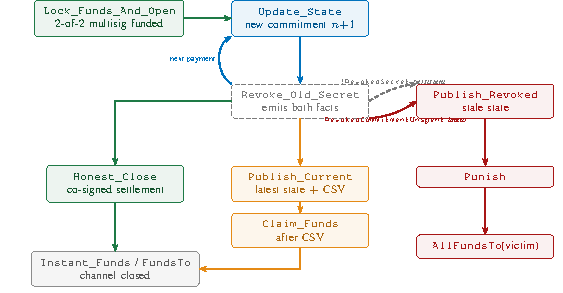
\includegraphics[width=\columnwidth,trim={0 40pt 0 0},clip]{figs/fig1_lifecycle.pdf}
  \caption{Channel lifecycle, labelled with the rules of our model.
    \textcolor{green!45!black}{Green}: opening and cooperative close;
    \textcolor{blue!70!black}{blue}: update loop;
    \textcolor{orange!90!black}{orange}: unilateral close with its CSV delay;
    \textcolor{red!75!black}{red}: revoked publish and punishment.
    \texttt{Revoke\_Old\_Secret} emits \emph{two} facts, and both gate
    punishment: the persistent \texttt{!RevokedSecret} (dashed, checked but
    never consumed) and the linear \texttt{RevokedCommitmentUnspent} (solid,
    consumed once); gating on the persistent fact alone would let the same
    revoked commitment be spent more than once (Sec.~\ref{sec:verified}).
    Grace-period and pending-publish paths, and the counterparty's instant
    output on a unilateral close, are elided.}
  \label{fig:lifecycle}
\end{figure}

\begin{figure}[t]
  \centering
  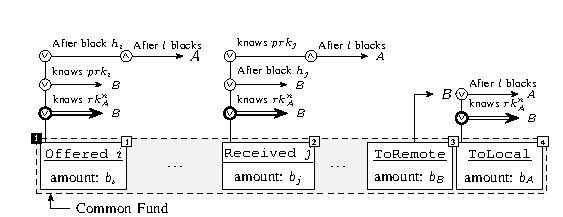
\includegraphics[width=\columnwidth]{figs/fig2_transaction.pdf}
  \caption{Commitment transaction held by $A$. The CSV is set to $l$, and the
    timeout (CLTV) of the $k$th HTLC is set to height $h_k$ for the
    \texttt{Offered} and \texttt{Received} outputs; $prk_k$ is the
    corresponding preimage of the payment hash; $\Rightarrow$ denotes the
    punishment path; and \txout{1} refers to an output.}
  \label{fig:transaction}
\end{figure}

The Payment Channel protocol fundamentally enables two agents to \emph{commit}
and \emph{revoke} a shared blockchain-related ``state''. This state typically
tracks the balance of some multi-sig~\cite{bip11} \emph{common fund},
effectively transferring coins between its two participants. The state is
represented by valid transactions spending that common fund, and a payment
channel ensures these transactions are valid and that no agent can publish an
old, favourable state. The latter property comes from careful signing
(restricting transactions to agreed-upon shapes) and \emph{punishing}: a
participant may unconditionally retrieve \emph{all} funds locked in a channel
if their counterparty puts an old state on chain.

In the context of the Lightning Network, the state also tracks in-flight
payments which will propagate further than this channel. These are carried by
\emph{hash time-locked contracts} (HTLCs). We discuss HTLCs fully in
Sec.~\ref{sec:routing}. The protocol relies on two things: careful handling of
revocation keys and careful handling of transaction signatures.
Fig.~\ref{fig:lifecycle} shows the channel lifecycle.

\subsubsection{The Transactions}\label{sec:transactions}
Although we abstract it away in our model, one should keep in mind the shape of
the transaction in the Lightning Network. Fig.~\ref{fig:transaction} gives the
shape of the commitment transaction held by Alice in an Alice-Bob channel. This
transaction notably enables unilateral closing. Outputs \txout{3} and \txout{4}
enable the simple redistribution of the common fund between Alice and Bob,
while Outputs \txout{1} and \txout{2} lock the funds of in-flight payments
specific to the Lightning Network.

The figure also illustrates the punishment mechanism: unlike Bob's
Output~\txout{3}, Alice needs to wait for a relative timelock (CSV; common
abbreviation for the \texttt{CheckSequenceVerify} opcode) before redeeming
Output~\txout{4}. That gives Bob the opportunity to redeem Output~\txout{4}
using Alice's \emph{revocation key} ($rk_A$). This revocation key is initially
hidden from Bob. Alice only releases it as a proof that she will not use a
given state. This mechanism enables declaring states as ``old''.

Fig.~\ref{fig:transaction} also describes the local mechanism for in-flight
payments. Output~\txout{1} (resp.~\txout{2}) captures in-flight funds flowing
towards Bob (resp.\ Alice). Besides the punishment mentioned above, these
outputs are further governed by \emph{payment hashes} and a timeout. To
\emph{fulfil} an in-flight transfer, the receiver (Bob in the case of
Output~\txout{1}) needs the preimage of the payment hash associated with that
transfer. To prevent funds from being locked up, the output effectively reverts
to a regular output once a block height is reached (e.g., $h_i$ for
Output~\txout{1}). This absolute timeout is set with CLTV (common abbreviation
for the \texttt{CheckLockTimeVerify} opcode). The real Lightning Network uses a
two-stage construction to separate the CLTV and CSV conditions;
Fig.~\ref{fig:transaction} collapses it into a single output per HTLC.

Our model keeps Outputs~\txout{3} and~\txout{4} and the revocation path, but
not the in-flight Outputs~\txout{1} and~\txout{2}: HTLCs are resolved in the
routing layer, and the single on-chain spend of an HTLC output becomes the
named assumption that each HTLC is resolved at most once
(Sec.~\ref{sec:method}).

\subsubsection{The Protocol}\label{sec:protocol}
The lifecycle of a channel has five phases: opening, update, revocation,
closing, and punishment, which correspond, left to right, to
Fig.~\ref{fig:lifecycle}.

\paragraph{Opening}\label{par:opening}
The opening phase aims to establish a first committed state and the common
fund, in that order, to prevent griefing attacks. After an unmodelled
negotiation of the inputs of the common fund, Alice and Bob each sample a
random revocation key ($rk^0_A$ and $rk^0_B$ respectively) and exchange their
hashes. Relying on SegWit~\cite{bip141}, both parties can compute the TXID of
the common fund and exchange the various signatures needed to spend it: the
common fund is an on-chain output locked by both parties with a 2-of-2
multisig~\cite{bip11}. For instance, Bob signs the various outputs of
Fig.~\ref{fig:transaction} (Sec.~\ref{sec:core-channels} describes how our
model abstracts these signatures). Then, the witnesses for the common fund are
exchanged and the funding transaction is published. Once it is on chain, the
channel is ready.

\paragraph{Update}\label{par:update}
The parties then pay each other off chain, by exchanging signed commitment
transactions. Updating involves setting up a new state, then revoking the old
one. The parties first commit to a new state via the same mechanism as in the
opening phase: sampling revocation keys ($rk^n_A$ and $rk^n_B$ respectively for
the $n$th state), exchanging their hashes, and exchanging the signatures. Only
then do they revoke the old state (here the $(n-1)$th state) by disclosing
their revocation keys to each other (e.g., $A$ sends $rk^{n-1}_A$ to $B$).
If the steps were reversed, a party would have nothing to publish. The old
state would be revoked, and the new one would not be signed. It could not close
the channel if the counterparty stopped responding.

\paragraph{Revocation}\label{par:revocation}
A state is retired by handing its revocation key to the counterparty: Alice
revokes state $n$ by giving $rk^n_A$ to Bob. The key is useless unless Alice
later publishes that state, at which point it lets Bob take the whole channel
balance. Revoking is therefore a proof of honesty, as publishing that old state
could then result in punishment. A commitment that has not been revoked yet is a valid unilateral close: either party may
publish it without penalty. Punishment is triggered only when a revoked
commitment is published.

\paragraph{Closing}\label{par:closing}
A channel can close in two ways. In the \emph{cooperative} close, the parties
agree on the final balance and sign one transaction together. This transaction
sends the final balance directly to their wallets. Only one on-chain
transaction is needed. There are no scripts and no delay. This is the cheapest
outcome for both. In a \emph{unilateral} close, either party can close: it
publishes its current commitment alone. The publisher's own output
(Output~\txout{4}) is restricted by the CSV delay and by the revocation path.
The party cannot spend its own output until the CSV delay ends. This delay
gives the counterparty time to check whether the published state was revoked:
if it was, the counterparty can take the output outright during that window.
The counterparty's own output (Output~\txout{3}) is spendable immediately.
Therefore, unilateral closing disadvantages the publisher and favours the
counterparty. This creates a punishment window, which is why an honest party
closes unilaterally only when its counterparty has stopped responding.

\paragraph{Punishment}\label{par:punishment}
If an old state is published on the blockchain by one party (i.e., a state
whose revocation key is known to the counterparty), the counterparty can defend
itself using the punishment paths shown in Fig.~\ref{fig:transaction} and claim
the entire channel balance. Punishment works as an \emph{active} defence: the
defender must act (i.e., notice the fraud, send the punishment transaction, and
wait for it to be accepted) within the window given by the CSV. Failure to
react makes the protocol trivially insecure~\cite{mccorry2019}.

\subsection{Multi-hop HTLC Routing}\label{sec:routing}

\begin{figure}[t]
  \centering
  \subfloat[Successful three-hop payment\label{fig:payment}]{%
    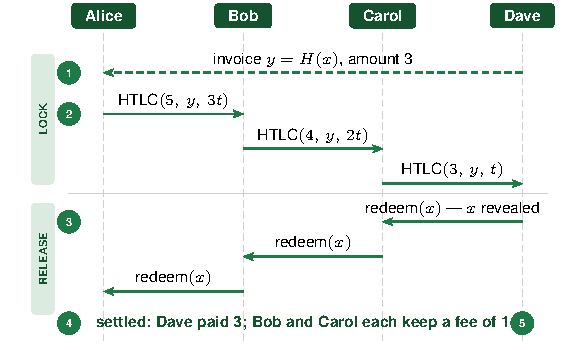
\includegraphics[width=\columnwidth]{figs/fig3a_payment.pdf}}\\[2pt]
  \subfloat[Griefing\label{fig:griefing}]{%
    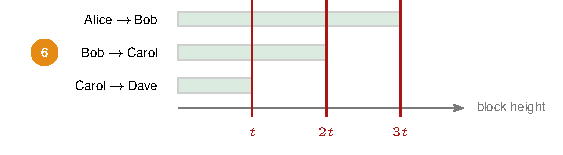
\includegraphics[width=\columnwidth]{figs/fig3b_griefing.pdf}}
  \caption{In-flight payments on the route Alice$\to$Bob$\to$Carol$\to$Dave.
    (a)~Amounts decrease $5\to4\to3$; each one-unit drop is that
    intermediary's fee. Deadlines decrease $3t > 2t > t$, so a forwarder whose
    outgoing HTLC is claimed still has time to redeem its incoming one.
    (b)~The HTLCs are locked as in (a), but Dave never releases $x$, so every
    HTLC runs to its deadline. Each window strictly contains the next. Capital
    is locked for the full window and the payment fails, but the nested
    deadlines $t < 2t < 3t$ mean that every honest party is refunded: griefing
    is a denial of service, not a loss of funds. Circled numbers index the
    lemma groups of Table~\ref{tab:groups}.}
  \label{fig:inflight}
\end{figure}

When the sender and recipient do \emph{not} share a direct channel, the payment
is routed through intermediaries along the path as in Fig.~\ref{fig:inflight}:
it is a \emph{multi-hop} payment. Because intermediaries are untrusted, each
hop relays the payment in an HTLC conditioned on a single shared secret, the
\emph{payment hash}. As a result, the payment is meant to either complete along
the entire path or fail. The wormhole attack (end of this section and
Sec.~\ref{sec:wormhole}) shows that colluding intermediaries can break this for
the hops between them. Furthermore, to provide an incentive, the
intermediaries are rewarded with a routing fee.

\begin{example}[Path]\label{ex:path}
We will use the running example where $S$ sends money to $R$ with the
following path:
\begin{equation}\label{eq:path}
  S \to F_1 \to \cdots \to F_n \to R
\end{equation}
\end{example}

\paragraph{Locking}
For this, the receiver ($R$ in Ex.~\ref{ex:path}) generates a preimage $x$ and
sends an invoice to the sender ($S$) containing the hash $y = H(x)$ and the
requested amount $v$, keeping $x$ strictly secret. The sender adds an HTLC to
its channel with $F_1$, locking funds $v_0$ on that channel conditional on $y$
before the deadline $d_0$; after $d_0$, the payer may reclaim them. The
condition to unlock the funds is to provide a preimage $x'$ with $H(x') = y$
before the deadline (as in Fig.~\ref{fig:transaction}). This moves forward
with each forwarder locking funds, the routing fee $v_{k-1} - v_k$ going to
forwarder $F_k$. Each HTLC uses the same hash but a decreasing deadline and
decreasing funds:
\begin{align}
  v_0 > v_1 > \cdots > v_n &= v \label{eq:amounts}\\
  d_0 > d_1 > \cdots > d_n & \label{eq:deadlines}
\end{align}
At this step, funds are still locked by the payment hash; they have not moved
yet. Each HTLC becomes an additional conditional output in the two parties'
current commitment transaction, as explained in Sec.~\ref{sec:channel}. The
intermediaries $F_i$ can safely lock funds, since an incoming HTLC has a larger
amount and a later deadline. If the outgoing HTLC is claimed, $F_i$ learns $x$
and still has time to unlock the incoming funds, keeping the difference as its
fee. Sec.~\ref{sec:core-amounts} explains how our model abstracts amounts and
deadlines.

\paragraph{Release Round}
In the release round, the receiver reveals $x$, the preimage, to the last
forwarder to claim the final HTLC. Since every HTLC has the same preimage, each
intermediary claims on its incoming channel using the same $x$, each learning
$x$ when the next hop claims from it. To claim $v_{n-1}$ from $F_{n-1}$, $F_n$
provides the secret $x$ for its incoming HTLC, and it keeps $v_{n-1} - v_n$ as
a fee. The preimage thus propagates backward hop by hop until the sender's HTLC
is settled. If any party in between fails to forward it and the timelock
expires, the funds return to the party that locked them. Once the receiver has
released $x$, if every intermediary claims its incoming HTLC in time, all HTLCs
on the path are settled. An intermediary that fails to do so after its
outgoing HTLC was redeemed loses the forwarded amount, while the parties
downstream are paid. This is why forwarders need liveness
(Remark~\ref{rmk:deadlines}).

\begin{remark}[Claiming and Liveness]\label{rmk:claiming}
Claiming can happen by mutual negotiation or by unilateral closing. Notably,
unilateral closing also publishes $x$, as it is leaked by the closing
transactions redeeming the HTLC.
\end{remark}

\begin{remark}[Decreasing Deadlines and Liveness]\label{rmk:deadlines}
Consider $F_i$ holding an incoming HTLC with deadline $d_{i-1}$ and an outgoing
HTLC with deadline $d_i$. If $F_{i+1}$ unilaterally claims the outgoing HTLC at
$d_i$, $F_i$ learns $x$ as late as $d_i$ and is left the window
$(d_i, d_{i-1})$ to settle its incoming HTLC. The gap between $d_{i-1}$ and
$d_i$ is the CLTV delta, which is precisely the time reserved for $F_i$ to
recover the funds. This means that, in case of unilateral close, forwarders
need liveness in order to claim their incoming HTLC within their claim
window~\cite{mccorry2019}.
\end{remark}

Our model imposes this liveness as an explicit restriction, T3
(Sec.~\ref{sec:restrictions}), and Sec.~\ref{sec:timing} shows that
intermediary safety fails without it.

Finally, all HTLCs of a payment are locked by the same hash $y$, so two
colluding intermediaries on the route can pass $x$ around the hops between
them: the payment completes while the bypassed hops are refunded and earn no
fee. This is the wormhole attack~\cite{malavolta2019}; Sec.~\ref{sec:wormhole}
gives such a trace, checked by \tamarin, and Sec.~\ref{sec:bypass} proves that,
for routes of any length, a hop of a settled payment whose hash is offered once
can be bypassed only if some party's long-term key is compromised.
